\titre{}
\theme{}
\auteur{Nathan Scheinmann}
\niveau{}
\source{}
\type{serie}
\piments{1}
\pts{}
\annee{2526}

\contenu{

  \qrcode{https://coopmaths.fr/alea/?uuid=8ff15&id=1mF2-10&n=3&d=10&s=2&s2=3&cd=1&lang=fr-CH&v=eleve&es=1211001}
	\tcblower

Déterminer les points d'intersection de ces trois droites.
\begin{center}
	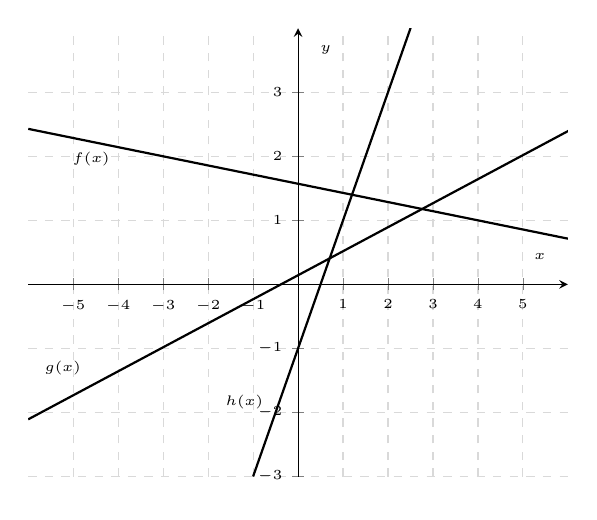
\begin{tikzpicture}[scale=1]
  \begin{axis}[
    axis lines=middle,
    xlabel={$x$}, ylabel={$y$},
    every axis x label/.style={at={(ticklabel* cs:0.92)}, anchor=west, yshift=10pt},
    every axis y label/.style={at={(ticklabel* cs:0.92)}, anchor=south, xshift=10pt},
    xmin=-6,   xmax=6,
    ymin=-3,   ymax=4,
    xtick={-5,-4,-3,-2,-1,0,1,2,3,4,5},
    ytick={-3,-2,-1,0,1,2,3},
    grid=both,
    grid style={dashed,gray!30},
    tick label style={font=\tiny},
    xlabel style={font=\tiny},
    ylabel style={font=\tiny}
  ]
    % branche pour x > 9
    \addplot[domain=-6:8, samples=200, thick]{-x*1/7+11/7}
      node[below,pos=0.1, font=\tiny] {$f(x)$};
    \addplot[domain=-6:8, samples=200, thick]{3/8*x+1/7}
      node[above left,pos=0.1, font=\tiny] {$g(x)$};
    \addplot[domain=-1:8, samples=200, thick]{2*x-1}
      node[above left,pos=0.05, font=\tiny] {$h(x)$};
  \end{axis}
\end{tikzpicture}
\end{center}
}
\correction{
	\tcblower

}
